\documentclass[11pt]{article}
\usepackage{fontspec}\setmainfont{Times New Roman}
\usepackage[paperwidth=595.32bp,paperheight=841.92bp,left=80bp,right=80bp,top=111bp,bottom=104bp]{geometry}
\usepackage{amsmath,amssymb,booktabs,longtable,array,pdfpages,hyperref,eso-pic,graphicx}
\hypersetup{hidelinks,pdftitle={BSE3124 Group 1 Answer Sheets v04}}
\pagestyle{empty}\setlength{\parindent}{0pt}\setlength{\parskip}{5pt}
\setlength{\tabcolsep}{4pt}\renewcommand{\arraystretch}{1.16}\emergencystretch=2em
\setlength{\unitlength}{1bp}
\newcommand{\slot}[4]{\put(#1,\dimexpr841.92bp-#2bp\relax){\makebox(0,0)[lt]{\begin{minipage}[t]{#3bp}\vspace{0pt}\fontsize{11}{13}\selectfont #4\end{minipage}}}}
\newcommand{\task}[1]{\section*{#1}}
\newcommand{\sheet}[2]{\long\gdef\currentsheetoverlay{#2}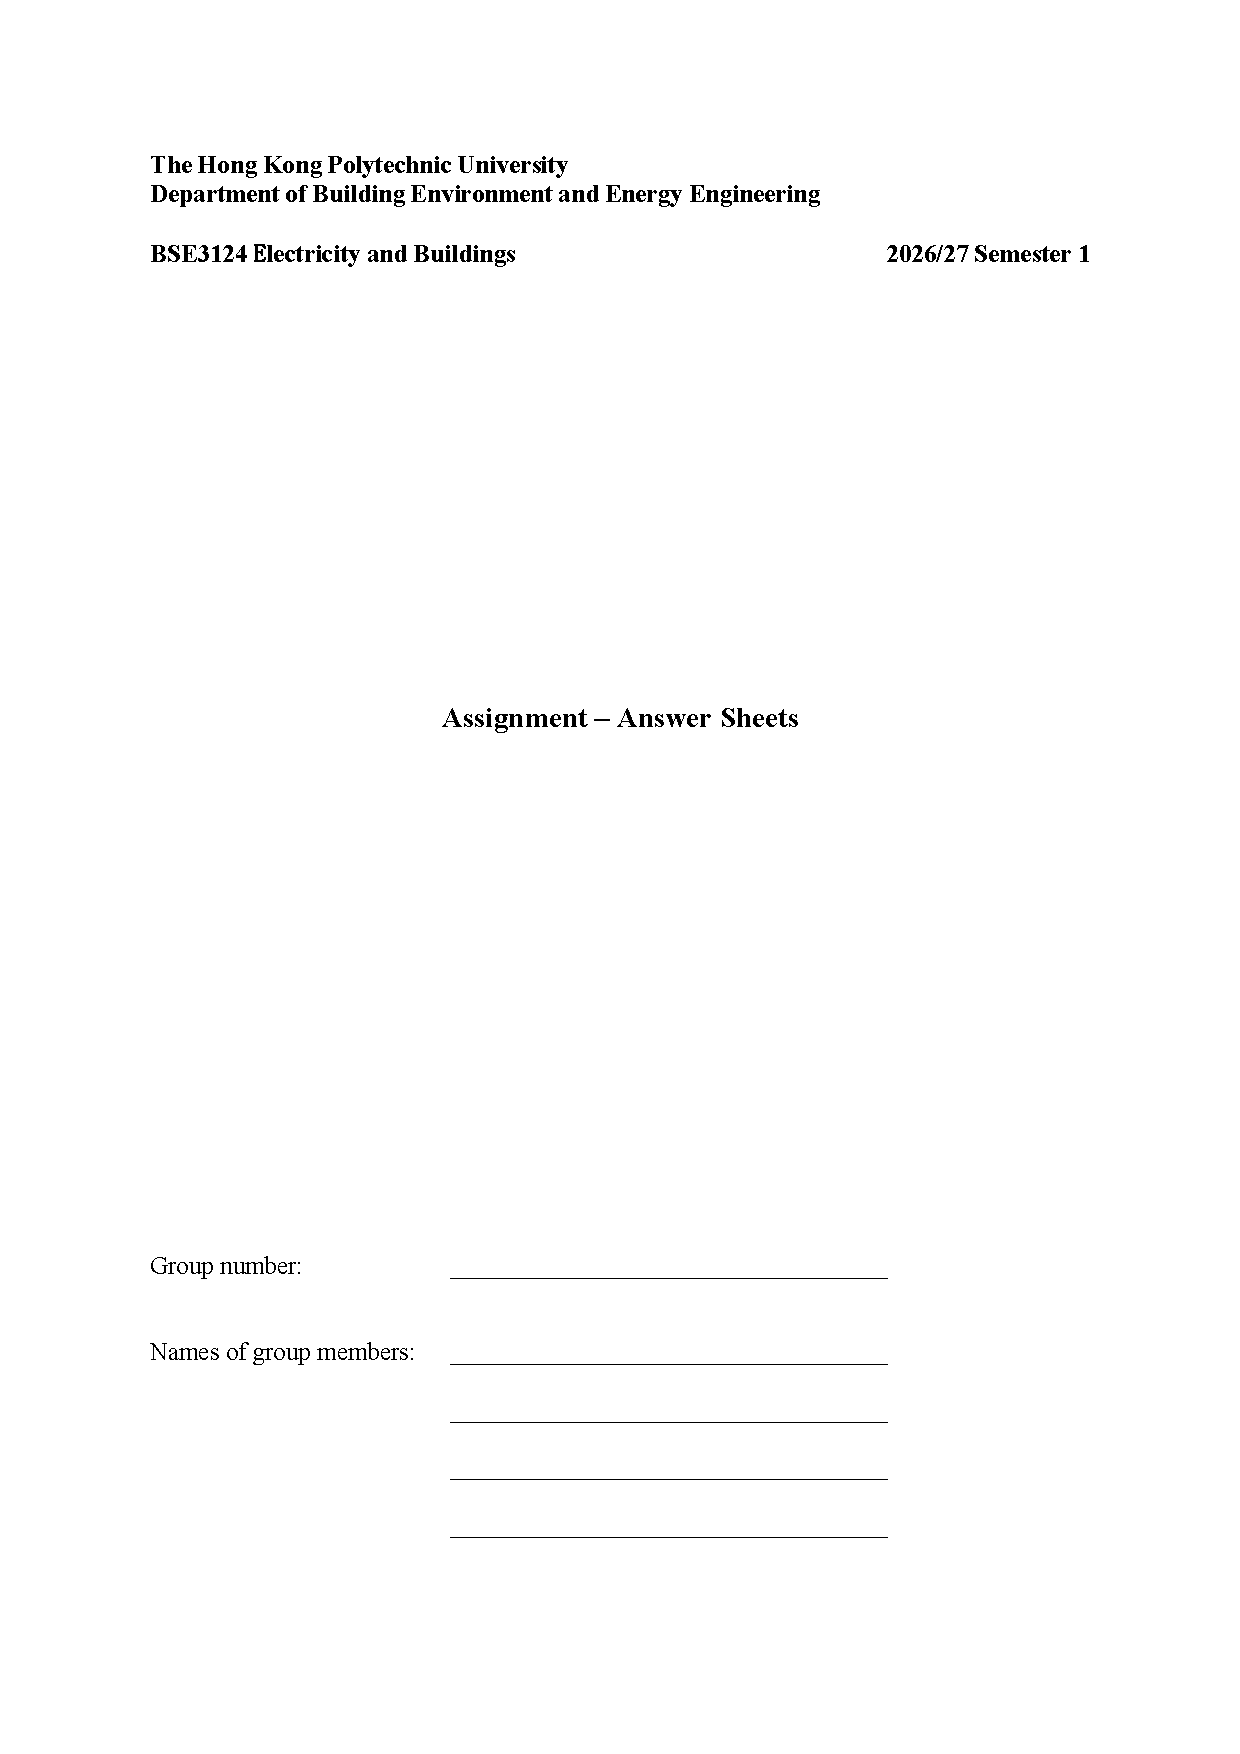
\includepdf[pages=#1,fitpaper=true,noautoscale=true,pagecommand={\AddToShipoutPictureFG*{\AtPageLowerLeft{\currentsheetoverlay}}}]{assets/official-template.pdf}}
\begin{document}
\sheet{1}{
\slot{220}{599}{205}{1}
\slot{220}{640}{205}{LYU Mingliang (24099296D)}
\slot{220}{668}{205}{HUANG Celine (24034414D)}
\slot{220}{696}{205}{LIU Wing Kei (24093229D)}}
\sheet{2}{\slot{80}{153}{435}{
\textbf{Basis and assumptions.} Ten identical office floors, each with usable areas assumed to be 309, 309 and 410\,m$^2$. Supplied CLP COP215 Rev07 is the course basis. The 1000\,kW in the question is cooling output, not electrical demand. Assume packaged air-cooled AC, PF 0.90, five lifts and equal allocation to two supply zones.
\begin{align*}
A&=10(309+309+410)=10\,280\ {\rm m^2},\\
S_{\rm office}&=10\,280(0.16)=1644.8\ {\rm kVA},\\
P_{\rm AC}&=(1000/3.51685)(1.85)=526.039\ {\rm kW},\\
S_{\rm AC}&=526.039/0.90=584.488\ {\rm kVA},\\
S_{\rm public}&=5(40)=200\ {\rm kVA},\\
S_{\rm design}&=1.10(1644.8+584.488+200)=2672.216\ {\rm kVA}.
\end{align*}
The 40\,kVA/lift allowance is an aggregate public-services reference, not a lift motor rating. A public-services overlap allowance of 0--200\,kVA gives 2452.216--2672.216\,kVA; adopt the upper bound. COP215: 3.1.7, 3.3.1 and Appendices 2/7.

\textbf{Selection.} Two 1500\,kVA transformers provide 3000\,kVA. Each serves five floors and half the plant/public allowance: 1336.108\,kVA per section. Full-load N--1 is not provided; a failed transformer requires load shedding. Prevent unauthorised parallel operation.

\textbf{Room location.} Use the lower-left ground-floor perimeter for the 12430$\times$5450\,mm transformer room and adjacent 12430$\times$3500\,mm main LV room (LV depth assumed). This allows external delivery/access, short LV interfaces, separation from the central lift/stair/AHU core and independent customer access.

Reserve 3\,m delivery access within 20\,m of unloading. Adopt COP101 v16 4.3 clearance envelopes, 2-hour partitions, sealed penetrations and raised floor level; these are planning conditions. Door sweeps require sequential use. Louvres provide 1.20\,m$^2$ free area at the assumed 50\% free ratio. Equipment/ventilation and 10.03/10.31\,m LV interfaces are detailed in the continuation and ground-floor drawings.
}}
\sheet{3}{\slot{80}{181}{435}{
\textbf{Selected tenant: Office 1.} See attached lighting/power plans, filled board template and detailed L/N/PE schematic.

\textbf{Lighting.} 92 PIL PLATO 600 panels: sixty 22\,W and thirty-two 28\,W, total 2216\,W. Seven circuits LC-A--LC-G have 18/17/18/11/14/10/4 lamps, each protected by B10 Type A 30\,mA 1P+N RCBO. Each has its own neutral and local manual control S-A--S-G. Different-phase switches use separate enclosures. Ceiling-grid and furniture relationships guide positions.

\textbf{Selection calculation.} Recalculation using the final device table and manufacturer LDT files gives mean maintained direct illuminance of 592.9/546.3/588.5/502.9\,lx for open office/pantry/upper east/south east. Adopt 1.9\,m luminaire-to-workplane height and MF 0.80. The south east room must not exceed this height without redesign; at 2.2\,m it falls below the 500\,lx target. The continuation records geometry, method, sensitivity and the limits of this average-illuminance check.

\textbf{Power.} Nine four-socket floorboxes, three twin sockets and FS01. Every assembly has one upstream 13\,A FCU; its outlets share that capacity. P1--P4: 6\,mm$^2$ A1 rings/B32; P5/P6/P8: 10\,mm$^2$ A2 radials/B32; P7: 4\,mm$^2$ dedicated radial/B16. Each local fused spur is 4\,mm$^2$, assumed 0.5\,m. FCUs precede the spur cable. Separate pantry circuits from ordinary office circuits. FS01 reserves 13\,A without inventing an appliance rating.

\textbf{Protection and containment.} Keep L/N/CPC ring continuity and return both ends to the same circuit. Apply EMSD Table 6(1)'s A1 conditions, not a fictitious ring-leg protective-device $I_2$. Separate the lighting group, ring banks A/B, radial bank C, P7 and incoming feeder so the stated grouping factors remain valid. See the new installation-detail sheet.

\textbf{Supply and controls.} Source C63 4P; 4C35\,mm$^2$ + CPC16; 100\,A 4P DB isolation. Dedicated neutrals pass through their own RCBO; PE is unswitched. Specify 10\,kA interruption and the stated total-energy/inrush limits. These are equipment selection requirements, not verified product certificates. Assume landlord emergency/exit systems on independent essential supplies; no normal panel is claimed as an emergency fitting.
}}
\sheet{4}{\slot{80}{139}{435}{
For lighting, $I=P/(220\times0.90)$. EMSD Table 7(1): take 90\% of lighting and 100\% of the largest Code 6E circuit plus 50\% of the remaining circuits on each phase. Reserve P7 at 100\% separately. The 13\,A per assembly is an intended maximum continuous load, not an instantaneous fuse clamp.
\begin{center}\begin{tabular}{lrrrr}\toprule
Phase & Light A$^*$ & Sockets A & Fixed A & Demand A\\\midrule
L1 & 3.444 & 45.500 & 0 & 48.600\\
L2 & 3.960 & 39.000 & 0 & 42.564\\
L3 & 3.788 & 32.500 & 13 & 48.909\\\bottomrule
\end{tabular}\end{center}
$^*$Lighting column is before the 90\% factor. Maximum demand is \textbf{48.909\,A}; select 63\,A source protection and 100\,A DB. Maximum undiversified phase allowance is 68.444\,A. Full branch currents are retained for outgoing cable sizing.
}
\slot{80}{402}{435}{
Select 4-core 35\,mm$^2$ PVC copper plus 16\,mm$^2$ CPC, Method B. Route 28.5119\,m plus assumed 3\,m vertical/termination allowance = 31.5119\,m. At 40\,$^\circ$C, $C_a=0.87$, $C_g=1$; adopt $C_h=0.86$ for the stated third-harmonic range (15--33\%).
\begin{align*}
I_{z,25}&=80(0.87)(0.86)=59.856<63\ {\rm A},\\
I_{z,35}&=99(0.87)(0.86)=74.0718\ {\rm A},\\
I_b&=48.909\le I_n=63\le I_z=74.0718\ {\rm A}.
\end{align*}
Ratings: EMSD A6(2), column 5. CPC: Table 11(2)(a). Full-size neutral retained; neutral current must remain within the adopted bound.

At 63\,A, feeder drop is 2.521606\,V. Add 2.2\,V pre-origin allowance and the calculated branch drops: worst complete drop 3.031\% of 220\,V, below 4\%. Adopt TN-S, source $Z_e=0.20\,\Omega$ and PFC $\le6$\,kA. Then DB external loop is 0.264129\,$\Omega$; source C63 disconnection and outgoing B-curve checks pass under those conditions.

\textbf{Outgoing circuits are also included}, as required by the assignment: all 15 sizes, currents, lengths, voltage drops, earth-fault checks and apparatus energy requirements are tabulated in the continuation. Original template headings do not limit the calculation to incoming cable only.
}}
\sheet{5}{\put(105,190){\rotatebox{90}{\begin{minipage}{450bp}\fontsize{9}{11}\selectfont\textbf{DB-O1: 8-way TPN chassis; 15 used single-phase outgoing positions}\par\smallskip\begin{tabular}{llll}\toprule Way & L1 & L2 & L3\\\midrule
1 & LC-A / B10 & LC-B / B10 & LC-C / B10\\
2 & LC-F / B10 & LC-E / B10 & LC-D / B10\\
3 & P1 / B32 & P3 / B32 & LC-G / B10\\
4 & P2 / B32 & P4 / B32 & P6 / B32\\
5 & P5 / B32 & Spare & P7 / B16\\
6 & Spare & Spare & P8 / B32\\
7 & Spare & Spare & Spare\\
8 & Spare & Spare & Spare\\
\bottomrule\end{tabular}\par\smallskip
Positions indicate phase allocation; each RCBO also needs its own N path. Confirm chassis/module capacity for 1P+N devices. Incoming: C63 4P at MS-O1; local main switch is 100A 4P (including N), supplementing the template's TP SW symbol. The detailed appended schematic governs neutral/PE connections and ring returns. All final RCBOs: Type A, 30mA, 10kA; see energy/inrush specifications.\end{minipage}}}}
\AddToShipoutPictureBG{\AtPageLowerLeft{\put(72.264,92.904){\linethickness{0.48bp}\framebox(450.916,649.156){}}\put(72.024,759){\fontsize{12}{14}\selectfont\bfseries BSE3124 -- Group 1 technical continuation}}}
\task{Task 1 Loading estimation and transformer room location}
\textbf{Technical continuation v04.} The original five-page template precedes this continuation. The stated assumptions define a course design, not site certification.
\subsection*{Building load assessment}
Adopt the drawing areas 309, 309 and 410\,m$^2$ as usable floor areas for ten identical office floors. This is a course assumption: the UFA exclusions have not been independently reconciled. Use supplied CLP COP215 Rev 07. The assignment's 1000\,kW is cooling capacity. Assume packaged air-cooled central AC, electrical PF 0.90 and five lifts. The 40\,kVA/lift public-services allowance is aggregate, not a lift motor rating.
\begin{align*}
A_{\rm UFA}&=10(309+309+410)=10\,280\ {\rm m^2},\\
S_{\rm office}&=10\,280(0.16)=1644.800\ {\rm kVA},\\
P_{\rm AC}&=\frac{1000}{3.51685}(1.85)=526.039\ {\rm kW},\\
S_{\rm AC}&=526.039/0.90=584.488\ {\rm kVA},\\
S_{\rm public}&=5(40)=200.000\ {\rm kVA}.
\end{align*}
COP215 Appendix 2 supplies the office density;  Appendix 7 supplies the AC reference. Public services follow clauses 3.1.6 and 3.3.1 and include lobby AC. Let $X$\,kVA be the duplicated AC share. Because it cannot exceed either overlapping allowance, $0\le X\le 200$. For the proposed two independent supply zones, apply clause 3.1.7:
\[
S_{\rm assessment}=1.1(1644.800+584.488+200-X).
\]
The range is 2452.216--2672.216\,kVA. Adopt the upper bound \textbf{2672.216\,kVA} for capacity reservation. This does not assert that actual overlap is zero. Do not add public lighting/pumps/fire-service allowances again on top of the aggregate reference.

\subsection*{Transformer and main LV room proposal}
Propose two 1500 kVA transformers with separate LV sections:3000 kVA total gives 327.784 kVA margin. Allocate floors 1--5 to A and 6--10 to B, each with half the central plant/public allowance. Each section is 1336.108 kVA, about 2030 A at 380 V. The equal split is assumed. Full-load N--1 is not provided;  load shedding is required on loss of one unit. Any coupler must prevent parallel operation.
Place the rooms at the lower-left perimeter of the supplied plan: substation 12430 by 5450 mm and adjacent LV room 12430 by 3500 mm, the latter depth assumed. Reasons are external plant access, short LV interfaces, separation from the lift/stair/AHU core and independent LV access. Reserve a 3 m delivery route within 20 m of unloading, subject to external site confirmation.
The appendix shows assumed HV3000 by 1000 mm and transformer 2200 by 1800 mm equipment reservations and six LV cabinets;  these are not manufacturer footprints. Their clearance envelopes fit without overlap. COP101 v 16 clause 4.3 requires HV rear 1000/front 1800/sides 750 mm and transformer LV terminals 900/others 750 mm. Propose 2-hour partitions, sealed penetrations and FFL150 mm above external level. Outward 180-degree doors have shared sweeps requiring sequential use.
Two 600 by 2000 mm louvres at assumed 50\% free area provide 1.20 m$^2$, above clause 6.3's 1.12 m$^2$ reference;  certified free area must be at least 46.67\%. Fan symbols are conditional provisions, not actual heat-loss calculations. LV interfaces including assumed tails are 10.03/10.31 m, below the 20 m limit in 5.5.2.2. Actual equipment, structures, openings and ventilation must satisfy these declared conditions.
\task{Task 2 Layout drawings and MCB board schematics}
\textbf{The office tenant chosen for layout design: Office 1.}
\subsection*{Normal lighting and local controls}
The design contains 92 working 600 mm-grid panel positions using PIL PLATO 600 MultiPower 3117955: sixty 22 W and thirty-two 28 W, total 2216 W. The retained LDT manifest gives nominal flux 2843.45 and 3555.30 lm respectively. Match the ceiling grid, partitions and furniture, with separate enclosed-space circuits and distributed main-office circuits. A500 lx task-plane target is a design assumption;  certified photometric uniformity/glare compliance is not claimed. Connected lighting density at the provisional 309 m$^2$ is 7.172 W/m$^2$;  this arithmetic alone is not energy-code compliance.
Seven local passive manual switches S-A--S-G control their corresponding circuits. Specify minimum 20AX, LED switching at least 600 W and make/break/inrush compatibility for the selected drivers. S-A/B/C use separate enclosures because their phases differ. No borrowed neutral is allowed. Routes visit each switch;  include 2 m DB rise plus 1.5 m down/1.5 m back at the switch, giving 5 m assumed vertical allowance per lighting radial. Passive controls add no operating power.
\begin{center}\begin{tabular}{lrrrrl}\toprule
Circuit & Lamps & W & Phase & RCBO & Control\\\midrule

LC-A & 18 & 402 & L1 & B10 & S-A \\
LC-B & 17 & 392 & L2 & B10 & S-B \\
LC-C & 18 & 396 & L3 & B10 & S-C \\
LC-D & 11 & 242 & L3 & B10 & S-D \\
LC-E & 14 & 392 & L2 & B10 & S-E \\
LC-F & 10 & 280 & L1 & B10 & S-F \\
LC-G & 4 & 112 & L3 & B10 & S-G \\

\bottomrule\end{tabular}\end{center}
Plan A/B/C numeric labels map to corresponding LED IDs and LC-A/B/C. D01--D11 map to PN01--PN11, E82--E96 excluding E90 to northeast LEDs, F01--F10 to UE01--UE10, G01--G04 to SE01--SE04. Power settings follow the common device schedule. Every luminaire and control has one circuit assignment.
\subsection*{Final lighting selection basis}
Use the final device table (92 panels, 2216 W), not legacy candidate schedules. Manufacturer LDT intensity is in cd/klm; scale by each selected setting's flux (22 W: 2843.45 lm; 28 W: 3555.30 lm). Integrating the intensity distribution confirms the parser's normalisation. At each 0.2 m grid cell, sum $E=I(C,\gamma)\cos\gamma/d^2$ and apply MF 0.80. No reflected-light contribution is counted.

Adopt 1.9 m between luminaires and the task plane, e.g. 2.7 m ceiling and 0.8 m workplane. Heights, periodic cleaning/replacement supporting MF, and room envelopes are explicit course assumptions. The connected main-office region and three side-room envelopes are drawn from retained geometry screens; their summed area is not the separate 309 m$^2$ UFA assumption. Lamps from other rooms are excluded.
\begin{center}\begin{tabular}{lrrrr}\toprule
Zone & Lamps & Area m$^2$ & Mean lx & Min/mean\\\midrule
Open office & 67 & 231.87 & 592.9 & 0.136\\
Pantry & 11 & 29.54 & 546.3 & 0.39\\
Upper east room & 10 & 33.68 & 588.5 & 0.267\\
South east room & 4 & 13.07 & 502.9 & 0.175\\
\bottomrule\end{tabular}\end{center}
All four adopted mean values meet the course target of 500 lx. At 2.2 m above the task plane, the means become 573.0, 505.8, 545.0 and 447.2 lx respectively. Therefore the south east room requires a height no greater than 1.9 m for this selection; do not assume 2.2 m is acceptable. Its margin is small, and changed dimensions or maintenance assumptions require recalculation.

Low perimeter minimum/mean ratios are disclosed, not called a uniformity pass. This average-illuminance selection check does not establish glare, furniture-shadow performance or maintained task-area uniformity. Those are distinct from the present course assumption. Reproduce with \texttt{final\_lighting\_basis.py}; the final lamp powers and counts are checked against the common table.

\subsection*{Small power and fixed equipment}
Provide nine four-socket floor boxes, three twin wall sockets and fixed connection FS01. Each floor-box/socket assembly is individually 13 A fused. This defines intended continuous demand, not an instantaneous current clamp. FS01 reserves equipment up to 13 A;  appliance identity/watts are not invented. Building central AC is supplied as central plant and not duplicated in this office DB.
P1--P4 are A1 rings with fused floor-box connections. P5/P6/P8 are A2 radials;  P7 is a fixed radial. Both P6 and P8 serve the source PANTRY;  including FB09 and SO01. P8 is retained as a separate socket group by design choice, not because each pantry outlet requires its own final circuit. Kitchen sockets are separated from ordinary office circuits under EMSD6E(3)(a).
\begin{center}\begin{tabular}{llllr}\toprule
Circuit & Points & Phase & Topology & Protection\\\midrule

P1 & FB01, FB02 & L1 & A1 ring & B32 \\
P2 & FB03, FB04 & L1 & A1 ring & B32 \\
P3 & FB05, FB06 & L2 & A1 ring & B32 \\
P4 & FB07, FB08 & L2 & A1 ring & B32 \\
P5 & SO02 & L1 & A2 radial & B32 \\
P6 & FB09, SO01 & L3 & A2 radial & B32 \\
P7 & FS01 & L3 & Fixed radial & B16 \\
P8 & SO03 & L3 & A2 radial & B32 \\

\bottomrule\end{tabular}\end{center}
Defined service envelopes satisfy A1 maximum 100 m$^2$ and A2 maximum 50 m$^2$. These are designed coverage polygons, not net UFA, with intentional overlap. Ring L/N/CPC return to their own circuit terminals. Main 6/10 mm$^2$ cables terminate in suitable accessible junction/FCU assemblies, not assumed ordinary socket terminals. Local connections use 4 mm$^2$ L/N/CPC and assumed 0.5 m per point.
\subsection*{FCU and containment details}
Every FB01--FB09 assembly shares one 13 A FCU upstream of all four socket ways. Each twin SO01--SO03 likewise shares one 13 A FCU; FS01 has its own switched 13 A FCU. Terminate ring/main L/N/CPC in an accessible junction assembly rated for 6/10 mm$^2$ cables. Put the FCU at the tap before the 4 mm$^2$ local spur; its neutral is switched with line, and PE is continuous. A fuse permits transient overcurrent: 13 A is the intended continuous capacity, not an instantaneous clamp. No additional unrecorded points are allowed without recalculation.

Containment banks: lighting LC-A--G (seven circuits, $C_g=0.54$); A: P1/P2 (four ring legs, 0.65); B: P3/P4 (four ring legs, 0.65); C: P5/P6/P8 (three radials, 0.70); P7 alone (1.00); incoming feeder alone (1.00). Co-located plan paths show routing corridors, not a shared enclosure. Provide separate Method B runs with horizontal clear space exceeding twice the largest adjacent overall cable diameter between groups, using EMSD A5(3), Note 2; where enclosure dimensions govern, space the enclosures at least as conservatively and confirm the cable separation. Do not treat a mere partition in one warm trunking as thermal separation. Each individual circuit's L/N/CPC stays together. Avoid thermal insulation contact. If these conditions cannot be achieved, regroup and resize before installation.

\subsection*{Protection and board arrangement}
The complete schematic shows C63 four-pole protection at MS-O1, 4-core 35 mm$^2$ plus CPC16, a 100 A four-pole DB isolator, independent L1/L2/L3/N/PE bars and 15 separate 1P+N TypeA30mA RCBOs. Every load neutral passes through its own RCBO;  none are shared downstream. PE bypasses all switches. Label circuits/phases and allow one final circuit to be isolated without interrupting the rest.
Use B-curve final protection and require compatible driver inrush. Do not change to a C curve without recalculation. Apparatus must meet Task 3 breaking/energy limits. Ratings/curves alone do not prove full short-circuit discrimination;  none is claimed.
\subsection*{Emergency lighting assumption}
Assume landlord emergency lighting/exit signage on independent essential systems, electrically separated under EMSD6B(4). No ordinary tenant panel is an emergency fitting. Emergency feeds must not pass through tenant normal-lighting switches or these RCBO load sides. Emergency load is excluded from this normal DB under this explicit course boundary;  installed escape coverage, autonomy and illuminance are not certified.
\task{Task 3 Maximum current demand calculation and cable sizing}
\subsection*{Maximum current demand}
For lighting, $I_b=P/(220\times 0.90)$. Incoming diversity follows EMSD Table 7(1):90\% of office lighting, and 100\% of the largest Code 6E circuit plus 50\% of the remaining circuit currents on each phase. Reserve P7 at 100\% separately. Use designed fused-point demand bounds, not breaker nameplates as appliance loads.
\begin{center}\begin{tabular}{lrrrr}\toprule
Phase & Lighting A & Socket demand A & P7 A & Total demand A\\\midrule

L1 & 3.444 & 45.500 & 0.000 & 48.600 \\
L2 & 3.960 & 39.000 & 0.000 & 42.564 \\
L3 & 3.788 & 32.500 & 13.000 & 48.909 \\

\bottomrule\end{tabular}\end{center}
Maximum phase demand is \textbf{48.909 A};  select C63 at the source and 100 A DB isolation/busbars. Maximum undiversified phase point allowance 68.444 A is below the board rating. This demand depends on the specified 13 A fused-point restrictions.
\subsection*{Incoming cable}
Select 4-core 35 mm$^2$ PVC copper L1/L2/L3/N plus separate 16 mm$^2$ PVC copper CPC, MethodB in protected enclosed containment. Proposed same-floor meter-to-DB route 28.5119 m plus assumed 3 m total vertical/termination allowance gives 31.5119 m. The proposed source is near the supplied METER label, not a measured termination. Upstream ground-to-floor distribution is retained through explicit voltage/fault conditions.
For 40\,degrees C take $C_a=0.87$, $C_g=1$, and $C_h=0.86$ for assumed third-harmonic content greater than 15\% and at most 33\% in this four-core cable (A5(7)). Keep a full-size neutral and reselect if this range is exceeded.
\begin{align*}
I_{z,25}&=80(0.87)(0.86)=59.856\,{\rm A}<63\,{\rm A},\quad\text{reject},\\
I_{z,35}&=99(0.87)(0.86)=74.0718\,{\rm A},\\
48.9091&\le63\le74.0718\,{\rm A},\quad\text{pass}.
\end{align*}
TableA6(2) column 5 supplies ratings. Table 11(2)(a) gives CPC16 for $16<S\le 35$;  energy is checked below. For unbalanced phase-neutral drop with neutral current at most 63 A, derive $(2/\sqrt 3)(1.10)=1.270170592$\,mV/A/m from the three-phase table impedance. Feeder drop at 63 A is 2.521606 V;  at design current 1.957610 V. This fundamental-frequency check is not harmonic-distortion assessment.
\subsection*{All outgoing cables}
All sizes are PVC copper L/N/CPC. Lighting grouped separately has $I_z=24(0.87)(0.54)=11.2752$A for seven 2.5 mm$^2$ circuits;  all $I_b\le 10\le I_z$. Lighting lengths include 5 m DB/switch vertical allowance.
Uniform ring banks count four current-carrying legs: $I_z=41(0.87)(0.65)=23.1855$A per 6 mm$^2$ leg, above the standard 20 A minimum. Ring-network solution at 13 A per point gives maximum leg currents 14.658--15.203 A, below $I_z$. Do not compare radial $I_n\le I_z$ against just one ring leg. Continuity and fused-point restrictions are essential.
The 10 mm$^2$ A2 radials have $I_z=57(0.87)(0.70)=34.713$A;  P7's separate 4 mm$^2$ radial has $I_z=32(0.87)=27.84$A. Power radial allowance is 2 m vertical, rings 2 m at each DB end;  all local point spurs add 0.5 m of 4 mm$^2$ cable.
\begin{longtable}{llrrrr}\toprule
Circuit & Phase & $I_b$ A & RCBO A & L/N/CPC mm$^2$ & Main length m\\\midrule\endhead

LC-A & L1 & 2.030 & 10 & 2.5 & 58.301 \\
LC-B & L2 & 1.980 & 10 & 2.5 & 62.184 \\
LC-C & L3 & 2.000 & 10 & 2.5 & 44.999 \\
LC-D & L3 & 1.222 & 10 & 2.5 & 27.233 \\
LC-E & L2 & 1.980 & 10 & 2.5 & 34.464 \\
LC-F & L1 & 1.414 & 10 & 2.5 & 32.710 \\
LC-G & L3 & 0.566 & 10 & 2.5 & 27.379 \\
P1 & L1 & 26.000 & 32 & 6 & 28.620 \\
P2 & L1 & 26.000 & 32 & 6 & 35.520 \\
P3 & L2 & 26.000 & 32 & 6 & 45.220 \\
P4 & L2 & 26.000 & 32 & 6 & 34.220 \\
P5 & L1 & 13.000 & 32 & 10 & 15.607 \\
P6 & L3 & 26.000 & 32 & 10 & 13.864 \\
P7 & L3 & 13.000 & 16 & 4 & 13.107 \\
P8 & L3 & 13.000 & 32 & 10 & 15.107 \\

\bottomrule\end{longtable}
\subsection*{Complete voltage drop and fault checks}
Sum segment downstream-current drops on radials and solve the two-feed ring network. Include stated vertical/local allowances. Add 2.2 V pre-origin allowance,2.521606 V feeder bound and outgoing drop. The full limit is $0.04(220)=8.8$V.
Adopt TN-S, external source loop impedance 0.20 ohm and PFC at most 6 kA at MS-O1/downstream. These are course conditions, not measurements. Incoming phase+CPC bound 0.064129 ohm gives DB external loop 0.264129 ohm. Table 11(10) reference limits are B10=4.17, B16=2.61, B32=1.31 and C63=0.33 ohm. Use operating-temperature paths and minimum voltage factor 0.95. Worst uniform-ring parallel path is at most quarter circumference.
\begin{longtable}{lrrrrr}\toprule
Circuit & Out drop V & Total drop \% & $Z_s$ ohm & Min fault A & $Z_s$ limit ohm\\\midrule\endhead

LC-A & 1.450 & 2.805 & 1.314 & 159.1 & 4.17 \\
LC-B & 1.237 & 2.709 & 1.383 & 151.1 & 4.17 \\
LC-C & 0.959 & 2.582 & 1.074 & 194.6 & 4.17 \\
LC-D & 0.422 & 2.338 & 0.754 & 277.1 & 4.17 \\
LC-E & 0.797 & 2.509 & 0.884 & 236.3 & 4.17 \\
LC-F & 0.642 & 2.438 & 0.853 & 245.0 & 4.17 \\
LC-G & 0.254 & 2.262 & 0.757 & 276.1 & 4.17 \\
P1 & 1.269 & 2.723 & 0.322 & 649.3 & 1.31 \\
P2 & 1.675 & 2.907 & 0.334 & 624.9 & 1.31 \\
P3 & 1.937 & 3.027 & 0.352 & 593.5 & 1.31 \\
P4 & 1.428 & 2.795 & 0.332 & 629.4 & 1.31 \\
P5 & 0.964 & 2.584 & 0.338 & 617.8 & 1.31 \\
P6 & 1.310 & 2.742 & 0.331 & 632.1 & 1.31 \\
P7 & 1.946 & 3.031 & 0.414 & 505.1 & 2.61 \\
P8 & 0.936 & 2.571 & 0.336 & 621.8 & 1.31 \\

\bottomrule\end{longtable}
All 15 full voltage bounds pass;  worst 3.031\%. Each B-curve final circuit exceeds minimum earth-fault threshold $5I_n$. Incoming C63 gives $Z_s=0.264129<0.33$ohm and $I_{f,\min}=791.28>10(63)=630$A, satisfying reference instantaneous disconnection under the adopted conditions.
\subsection*{Overload and total clearing energy}
Use $k=115$ for bunched PVC copper CPCs initially 70\,degrees C (11(2)(c));  require total $I^2t\le(kS)^2$. Specify 10 kA main/RCBO interruption. Require class 3-equivalent B-curve total energy at most 70,000 A$^2$s for B10/B16,90,000 for B32. These are functional selection requirements, not automatic certification of any RCBO. CPC withstands are 82,656.25 (2.5 mm$^2$),211,600 (4),476,100 (6),1,322,500 (10), each above the required device bound.
Incoming C63 total energy must be at most 1,000,000 A$^2$s over the relevant fault range, below CPC16 withstand 3,385,600. Complete 13 A FCU energy must be at most 90,000, below the 4 mm$^2$ spur withstand 211,600. The incoming/FCU limits are explicit apparatus performance specifications, not invented manufacturer data.
For fuse overload, $I_2=1.9(13)=24.7$A. Spur $I_z=32(0.87)(0.70)=19.488$A gives $1.45I_z=28.2576>24.7$A. For P1--P4, overload suitability uses the standard A1 arrangement in EMSD 6C, 6E and Table 6(1), Note 1(i): 32 A protection, copper size at least 2.5 mm$^2$, corrected per-leg capacity at least 20 A, served area at most 100 m$^2$, intact L/N/CPC rings and evenly distributed outlets. The adopted 6 mm$^2$ rings meet these conditions. Exactly two individually 13 A fused connections are allowed per ring; no extra unfused taps. The nominal leg-current solution is supplementary load-distribution evidence, not a protective-device $I_2$. The fuse reference 6 kA interruption meets assumed PFC at most 6 kA. Its typical pre-arcing 870 A$^2$s is \emph{not} total clearing energy. Assume FCU ambient at most 35\,degrees C and board apparatus at most 30\,degrees C;  containment 40\,degrees C remains the conservative cable condition.
\subsection*{Sources and reproducibility}
Cite supplied COP215 Rev 07 and downloaded COP101 v 16 as above. EMSD Wiring CoP2025: Table 6(1), printed 56/PDF 57; 7(1), printed 65--67/PDF 66--68; 9B, printed 79/PDF 80; 11(2), printed 99--100/PDF 100--101; 11(10), printed 105/PDF 106;  A5 factors PDF 274--279;  A6 tables PDF 282--285.
ABB guide 9AKK108468A3912 printed 130 gives the class 3 B-curve energy references. Eaton TDC180 Technical Data 2042 August 2024 p 2 gives conventional-fusing/interruption references, not total energy. URLs and explicit conditions are in the common data file \texttt{fault\_design\_conditions.json}.
Tables are generated from current common CSV/JSON data. Reproduce the lighting/power route, demand, incoming and fault scripts before rebuilding this answer. Guarded DWG mutations must not be rerun blindly. Original source documents are retained. Normal lighting/power layout PDFs have been visually reviewed. Final native DWG save/reopen consistency verification is recorded separately in the acceptance evidence.
\paragraph*{Drawing appendix}
The following sheets show the ground-floor proposal, complete Office 1 DB schematic, normal lighting plan and power plan. Print at actual size to preserve the stated drawing scales. Group 1 identities are shown on the official cover.
\clearpage\ClearShipoutPictureBG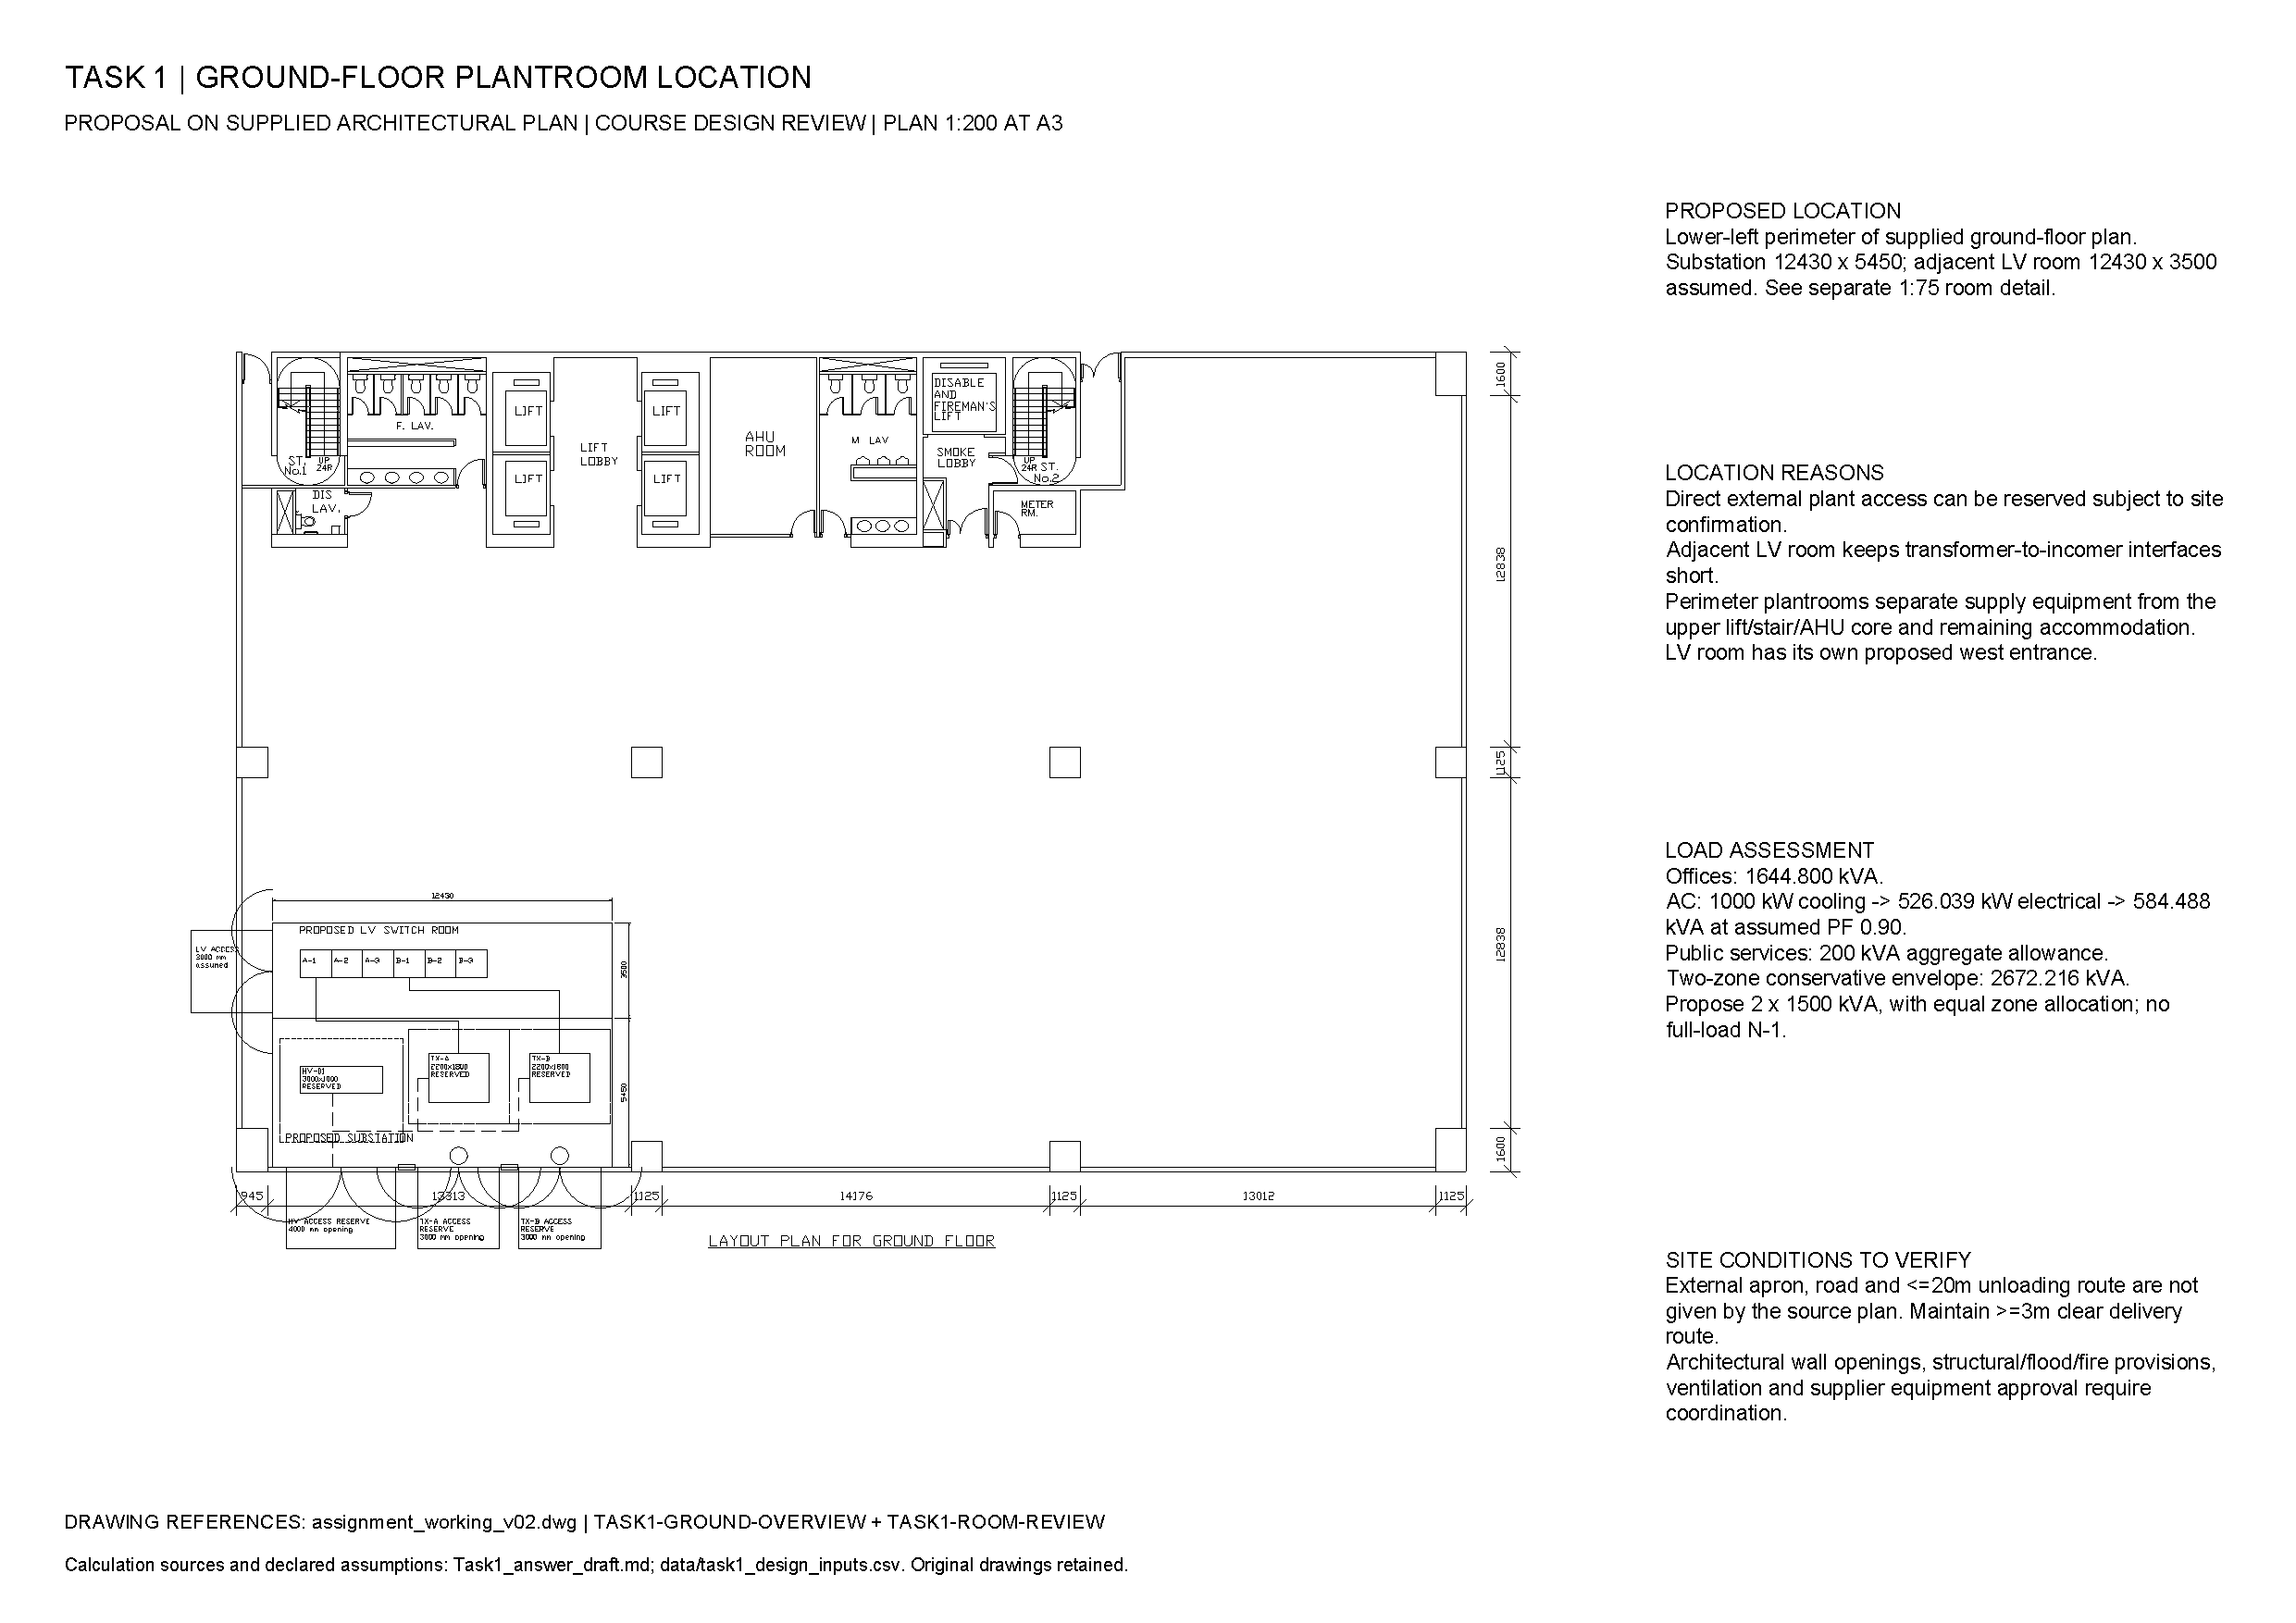
\includepdf[pages=-,fitpaper=true]{assets/task1-drawings.pdf}
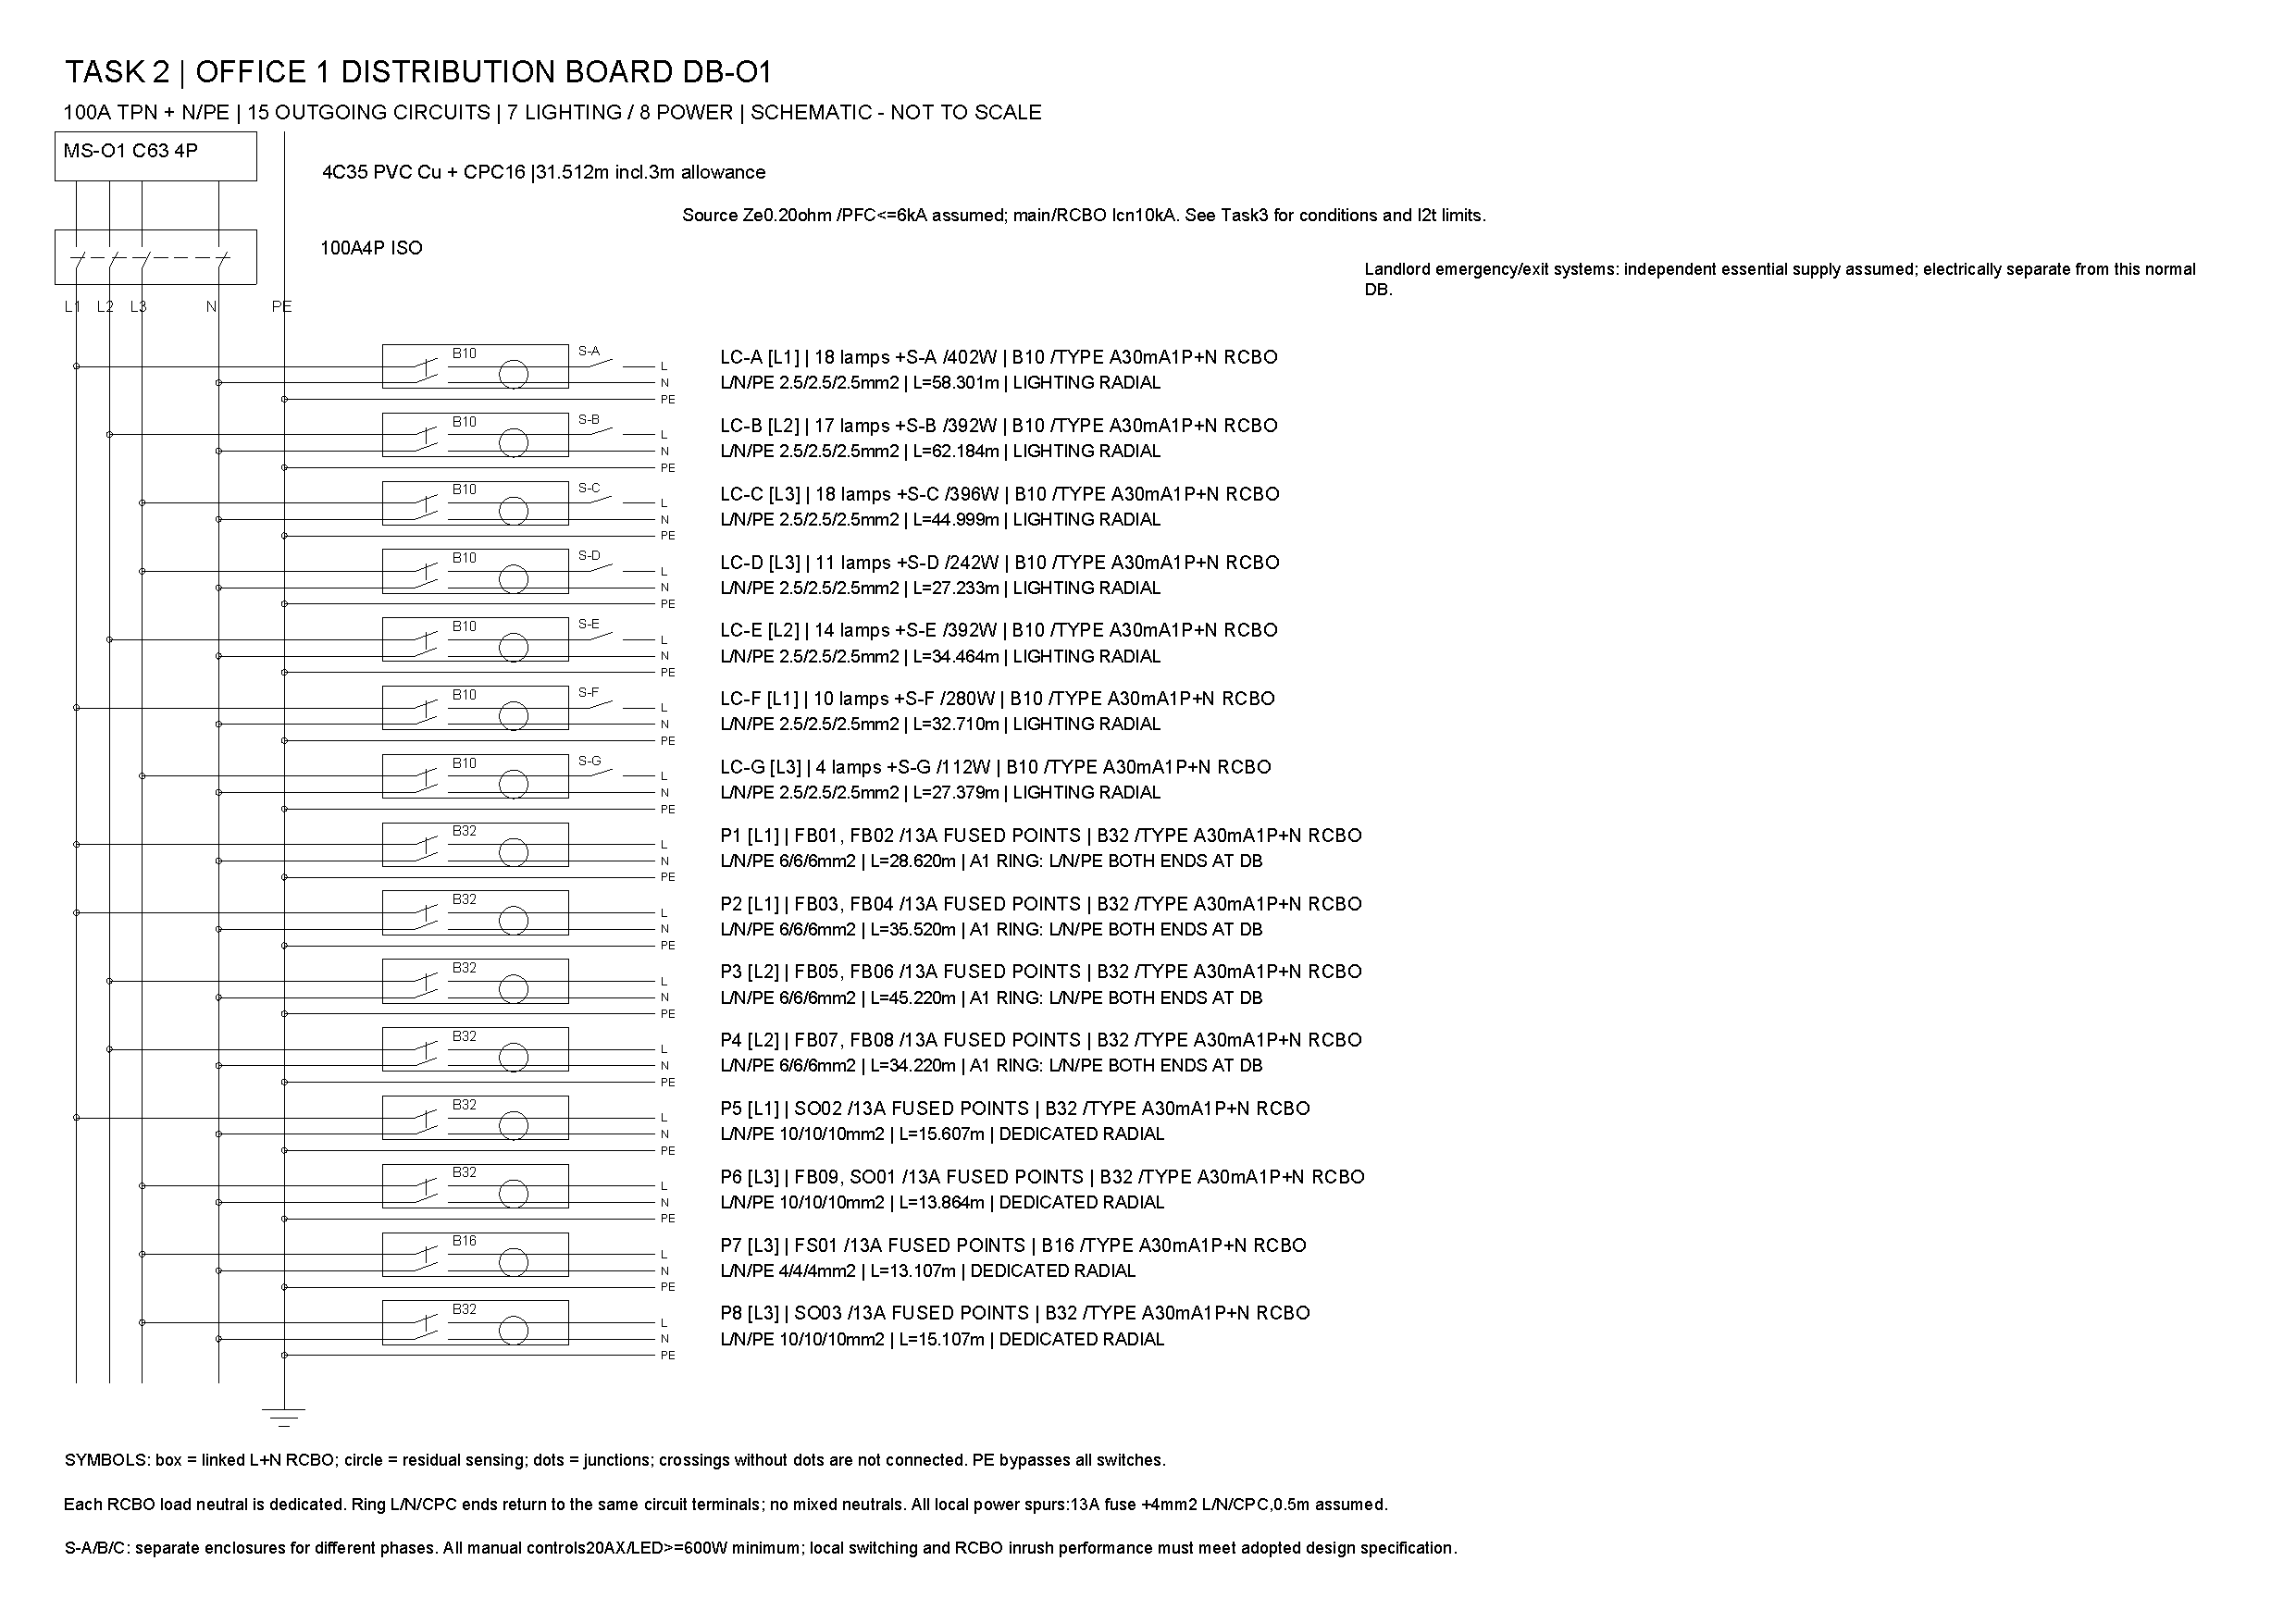
\includepdf[pages=-,fitpaper=true]{assets/office-db.pdf}
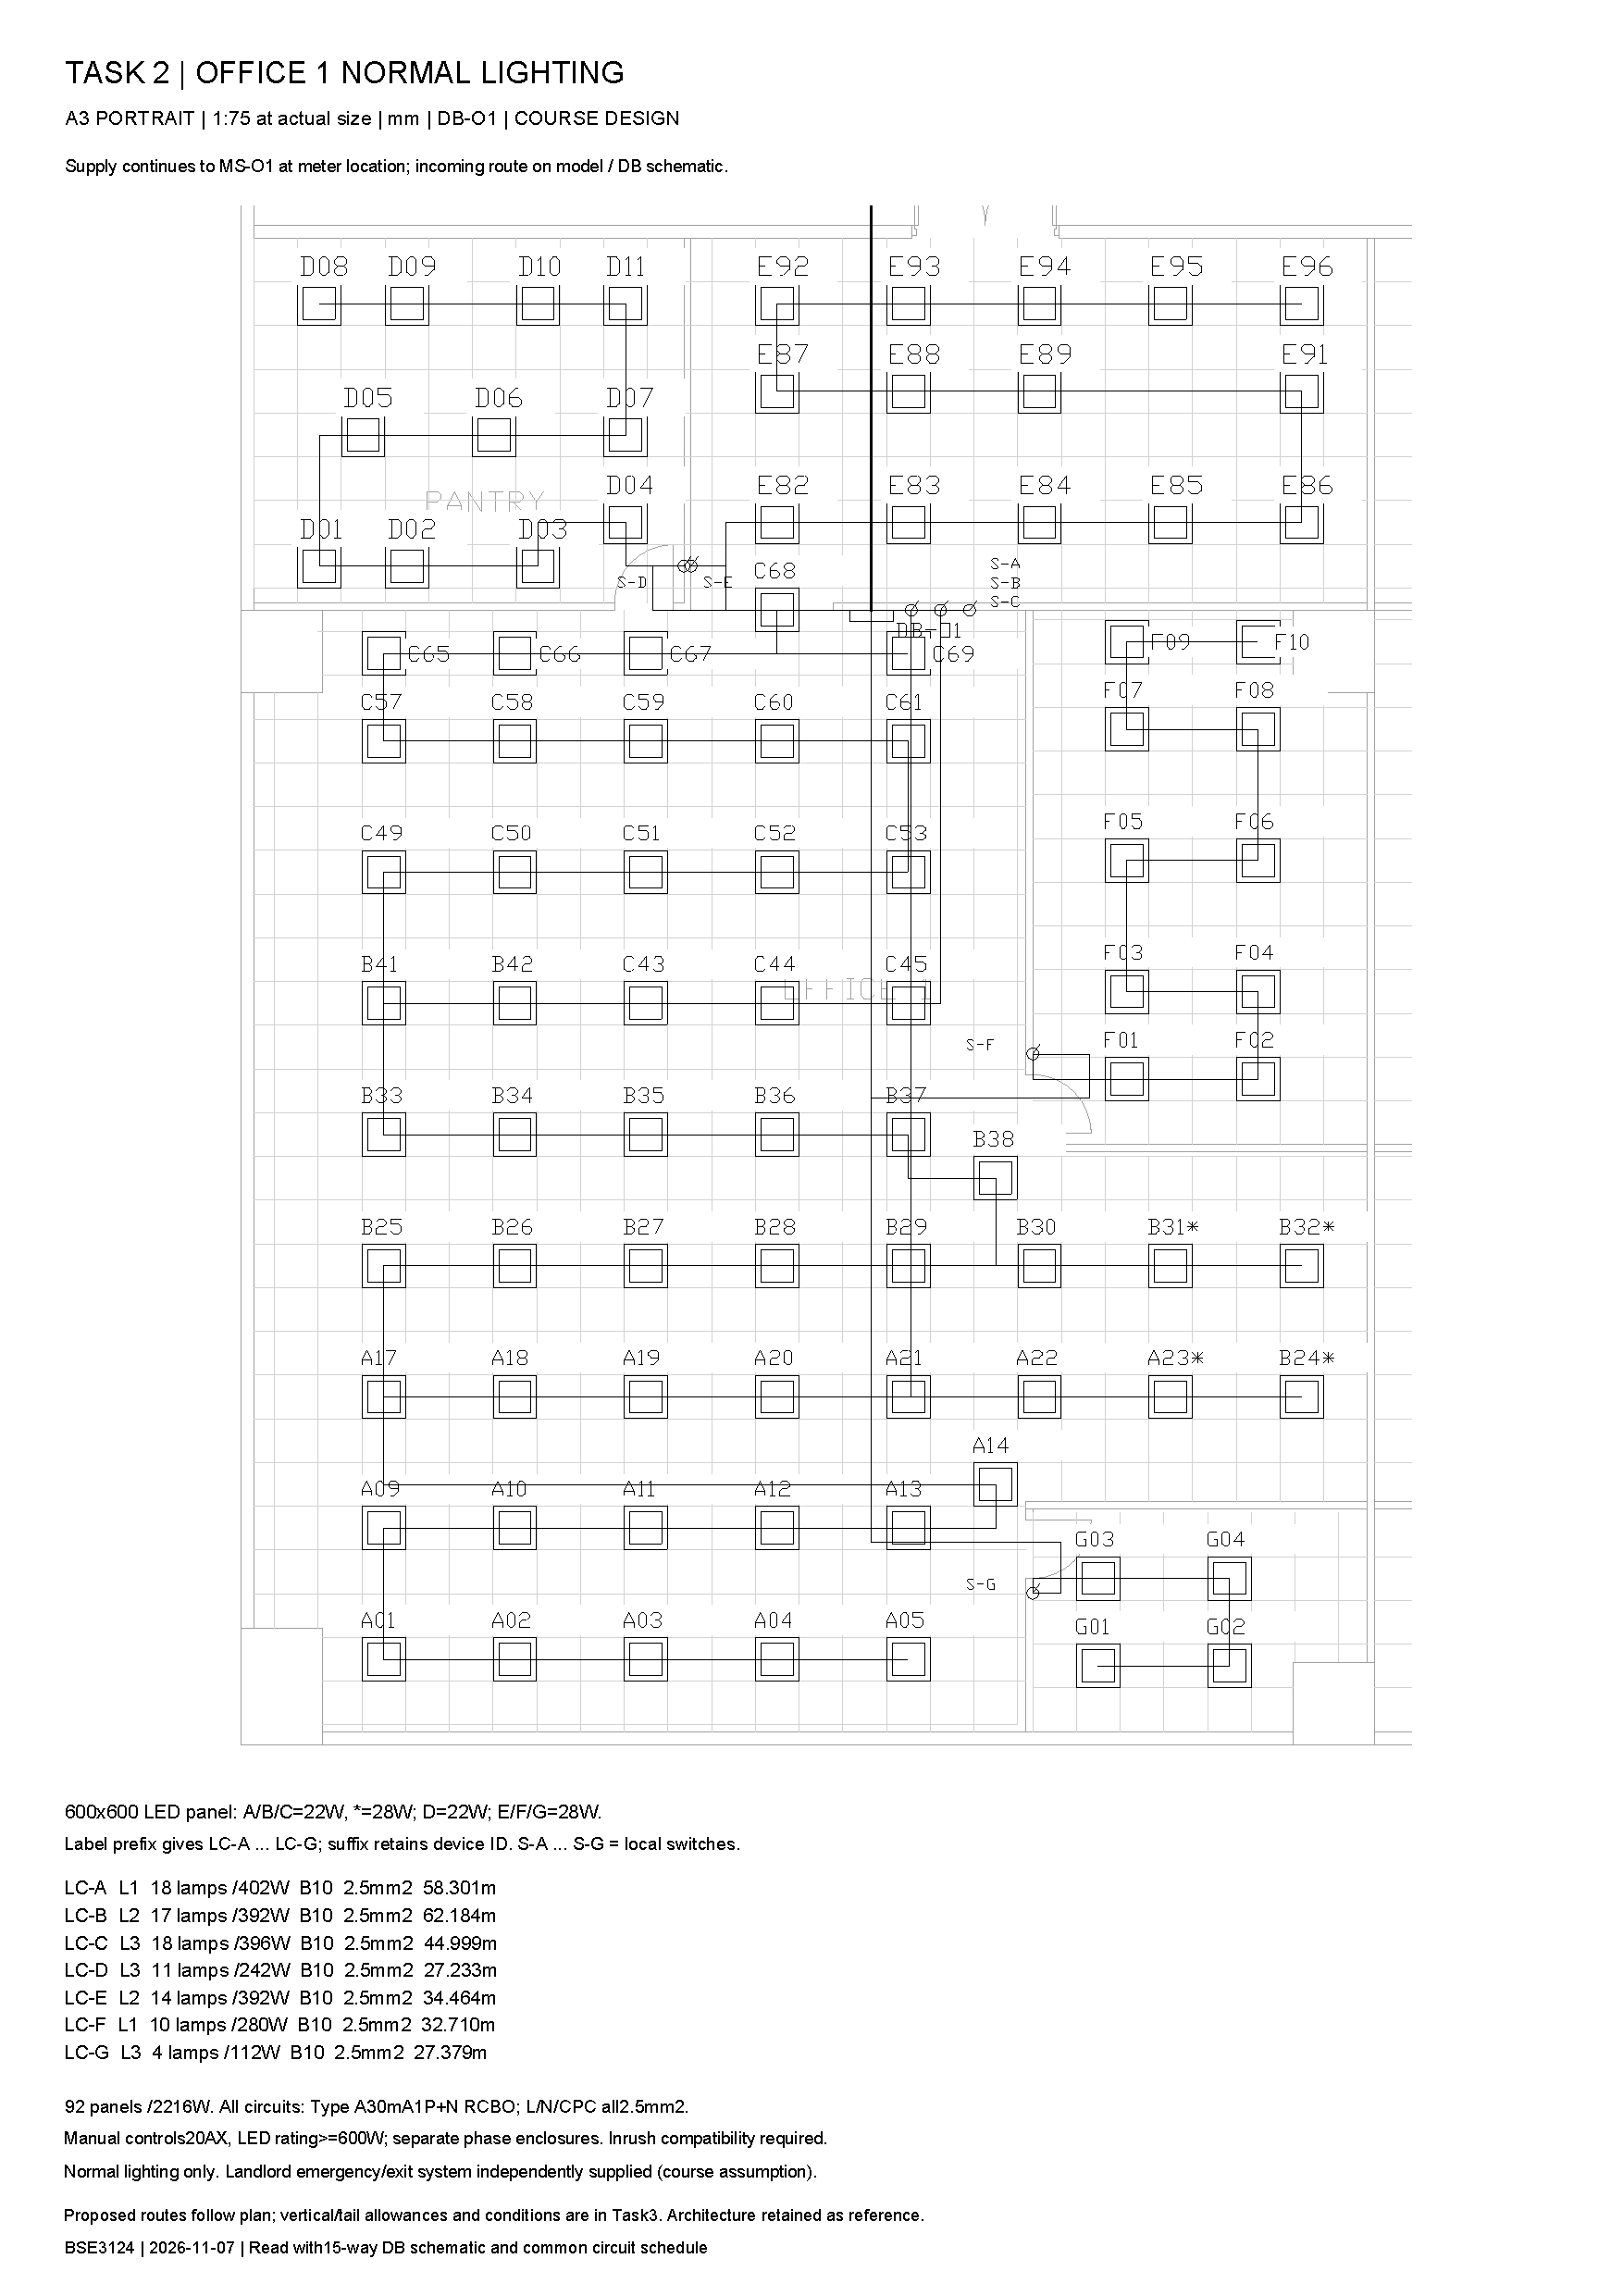
\includepdf[pages=-,fitpaper=true]{assets/office-lighting.pdf}
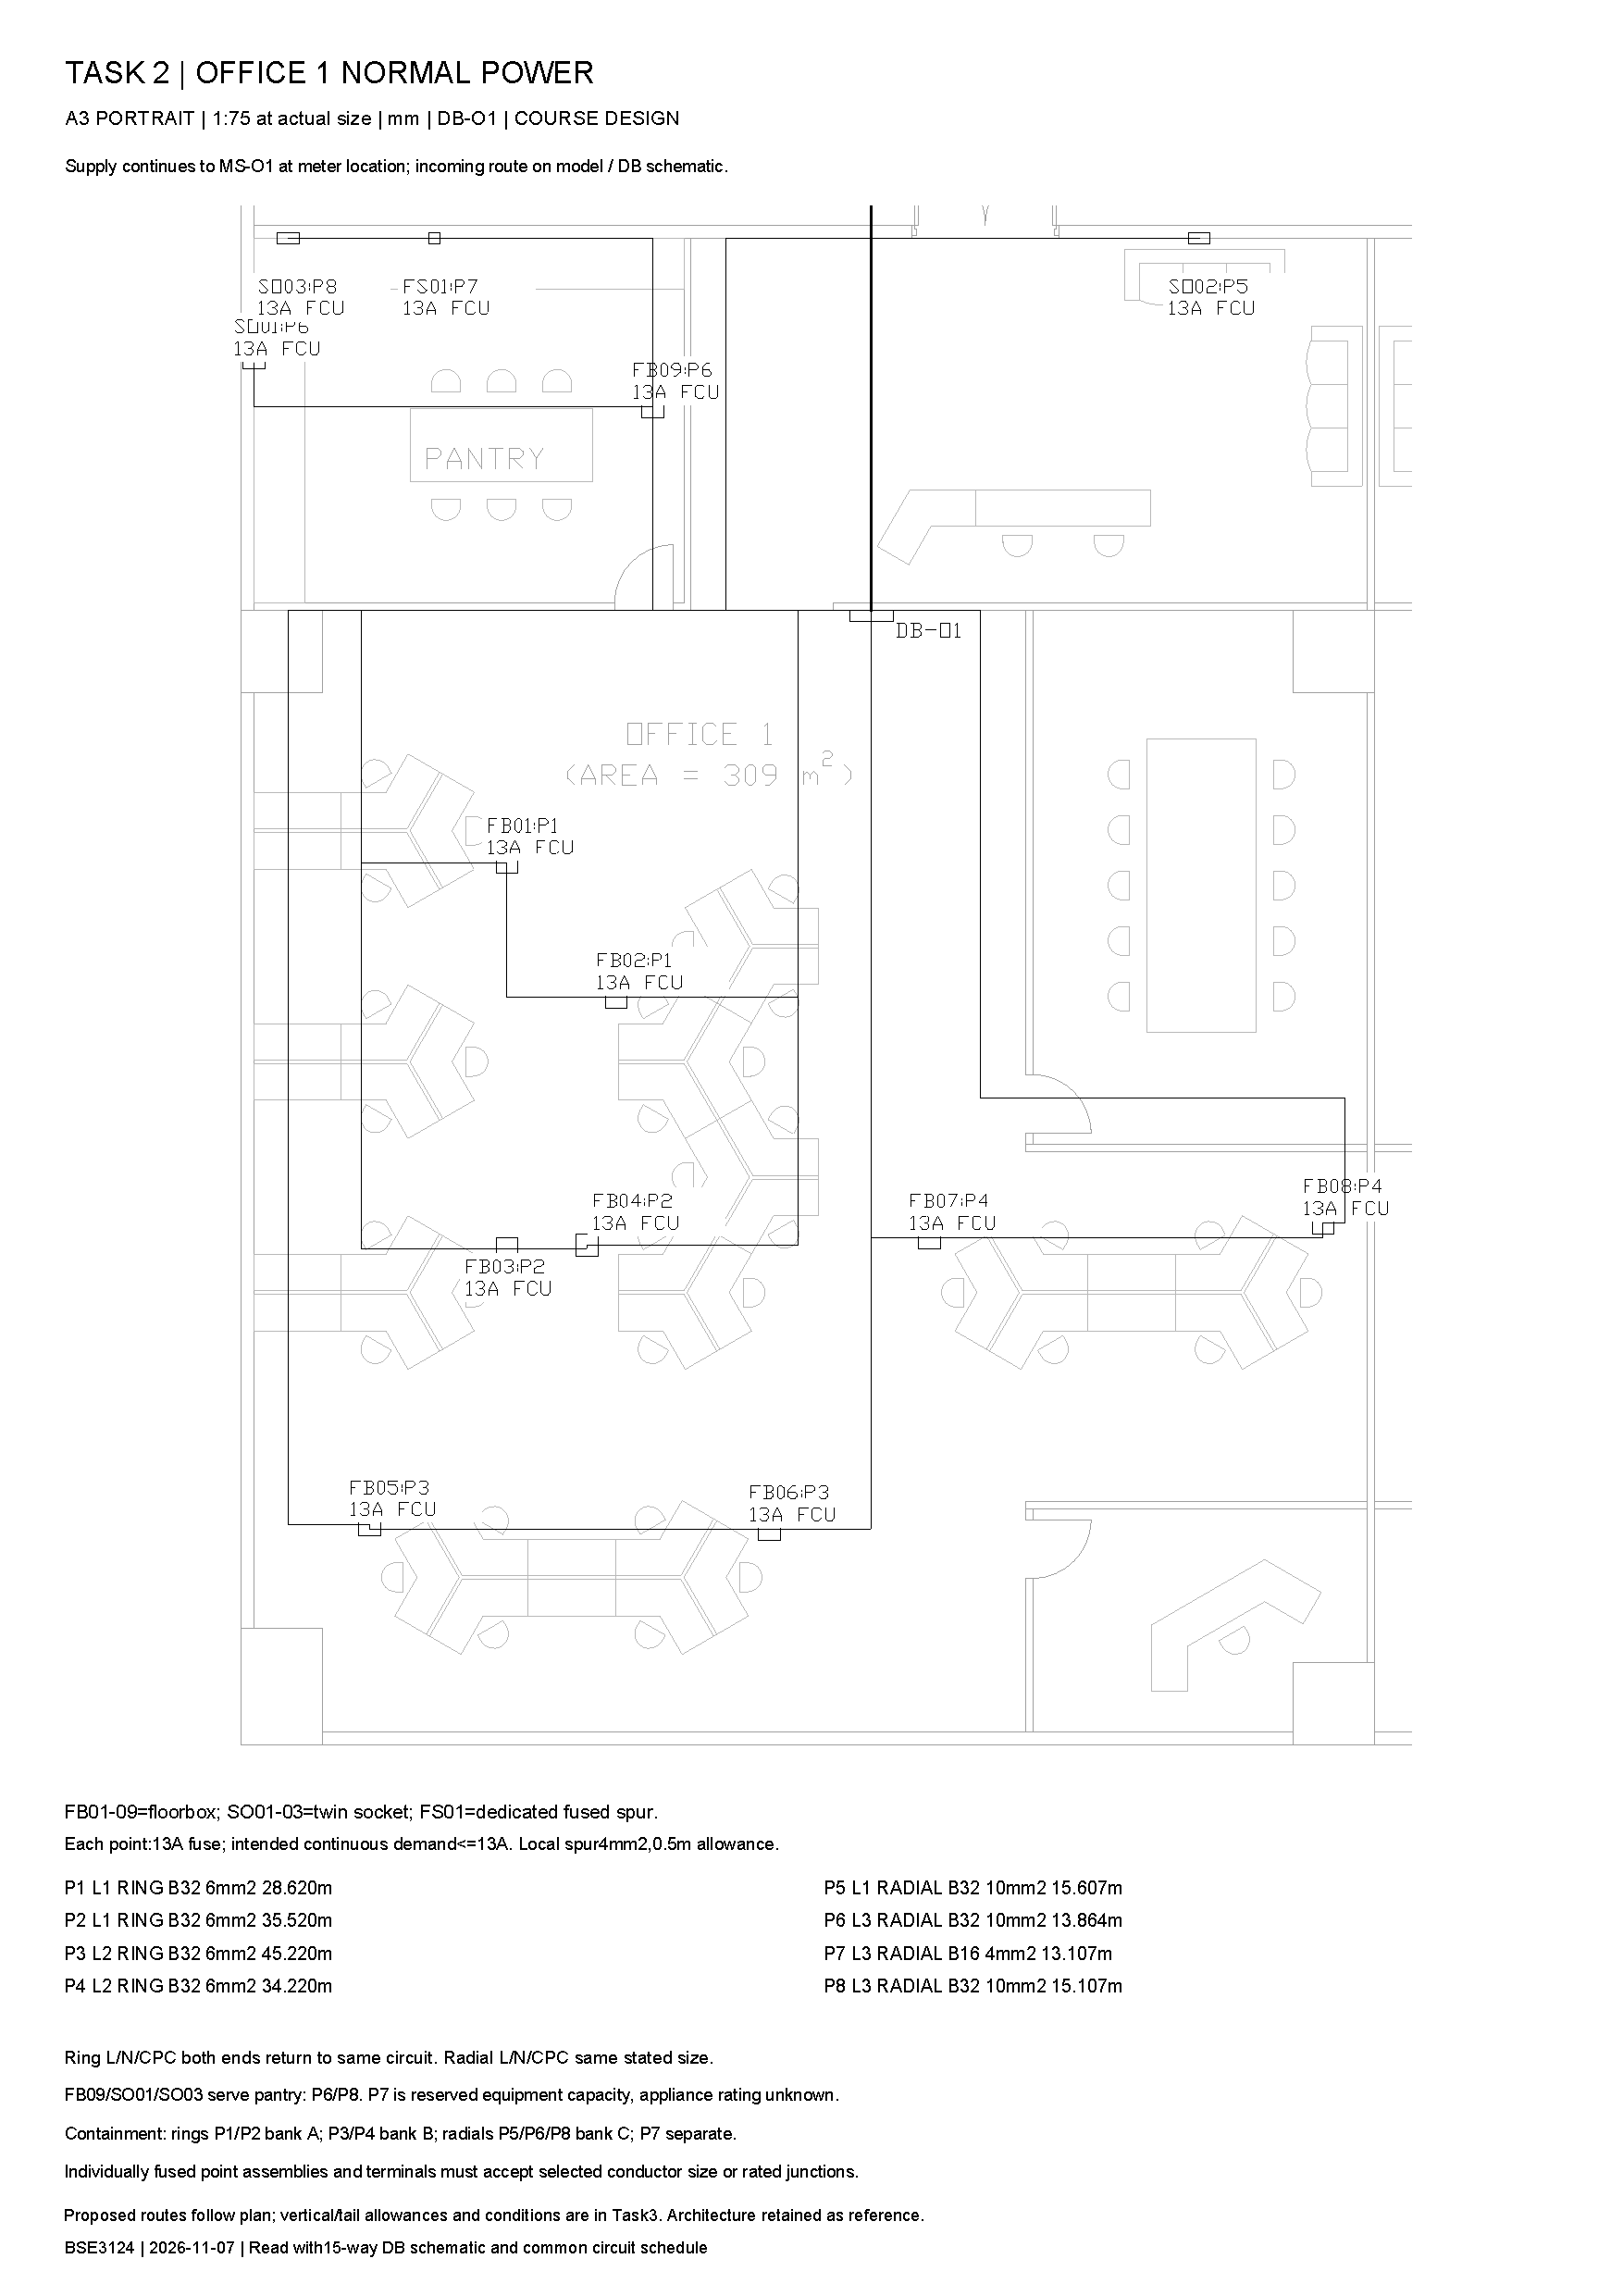
\includepdf[pages=-,fitpaper=true]{assets/office-power.pdf}
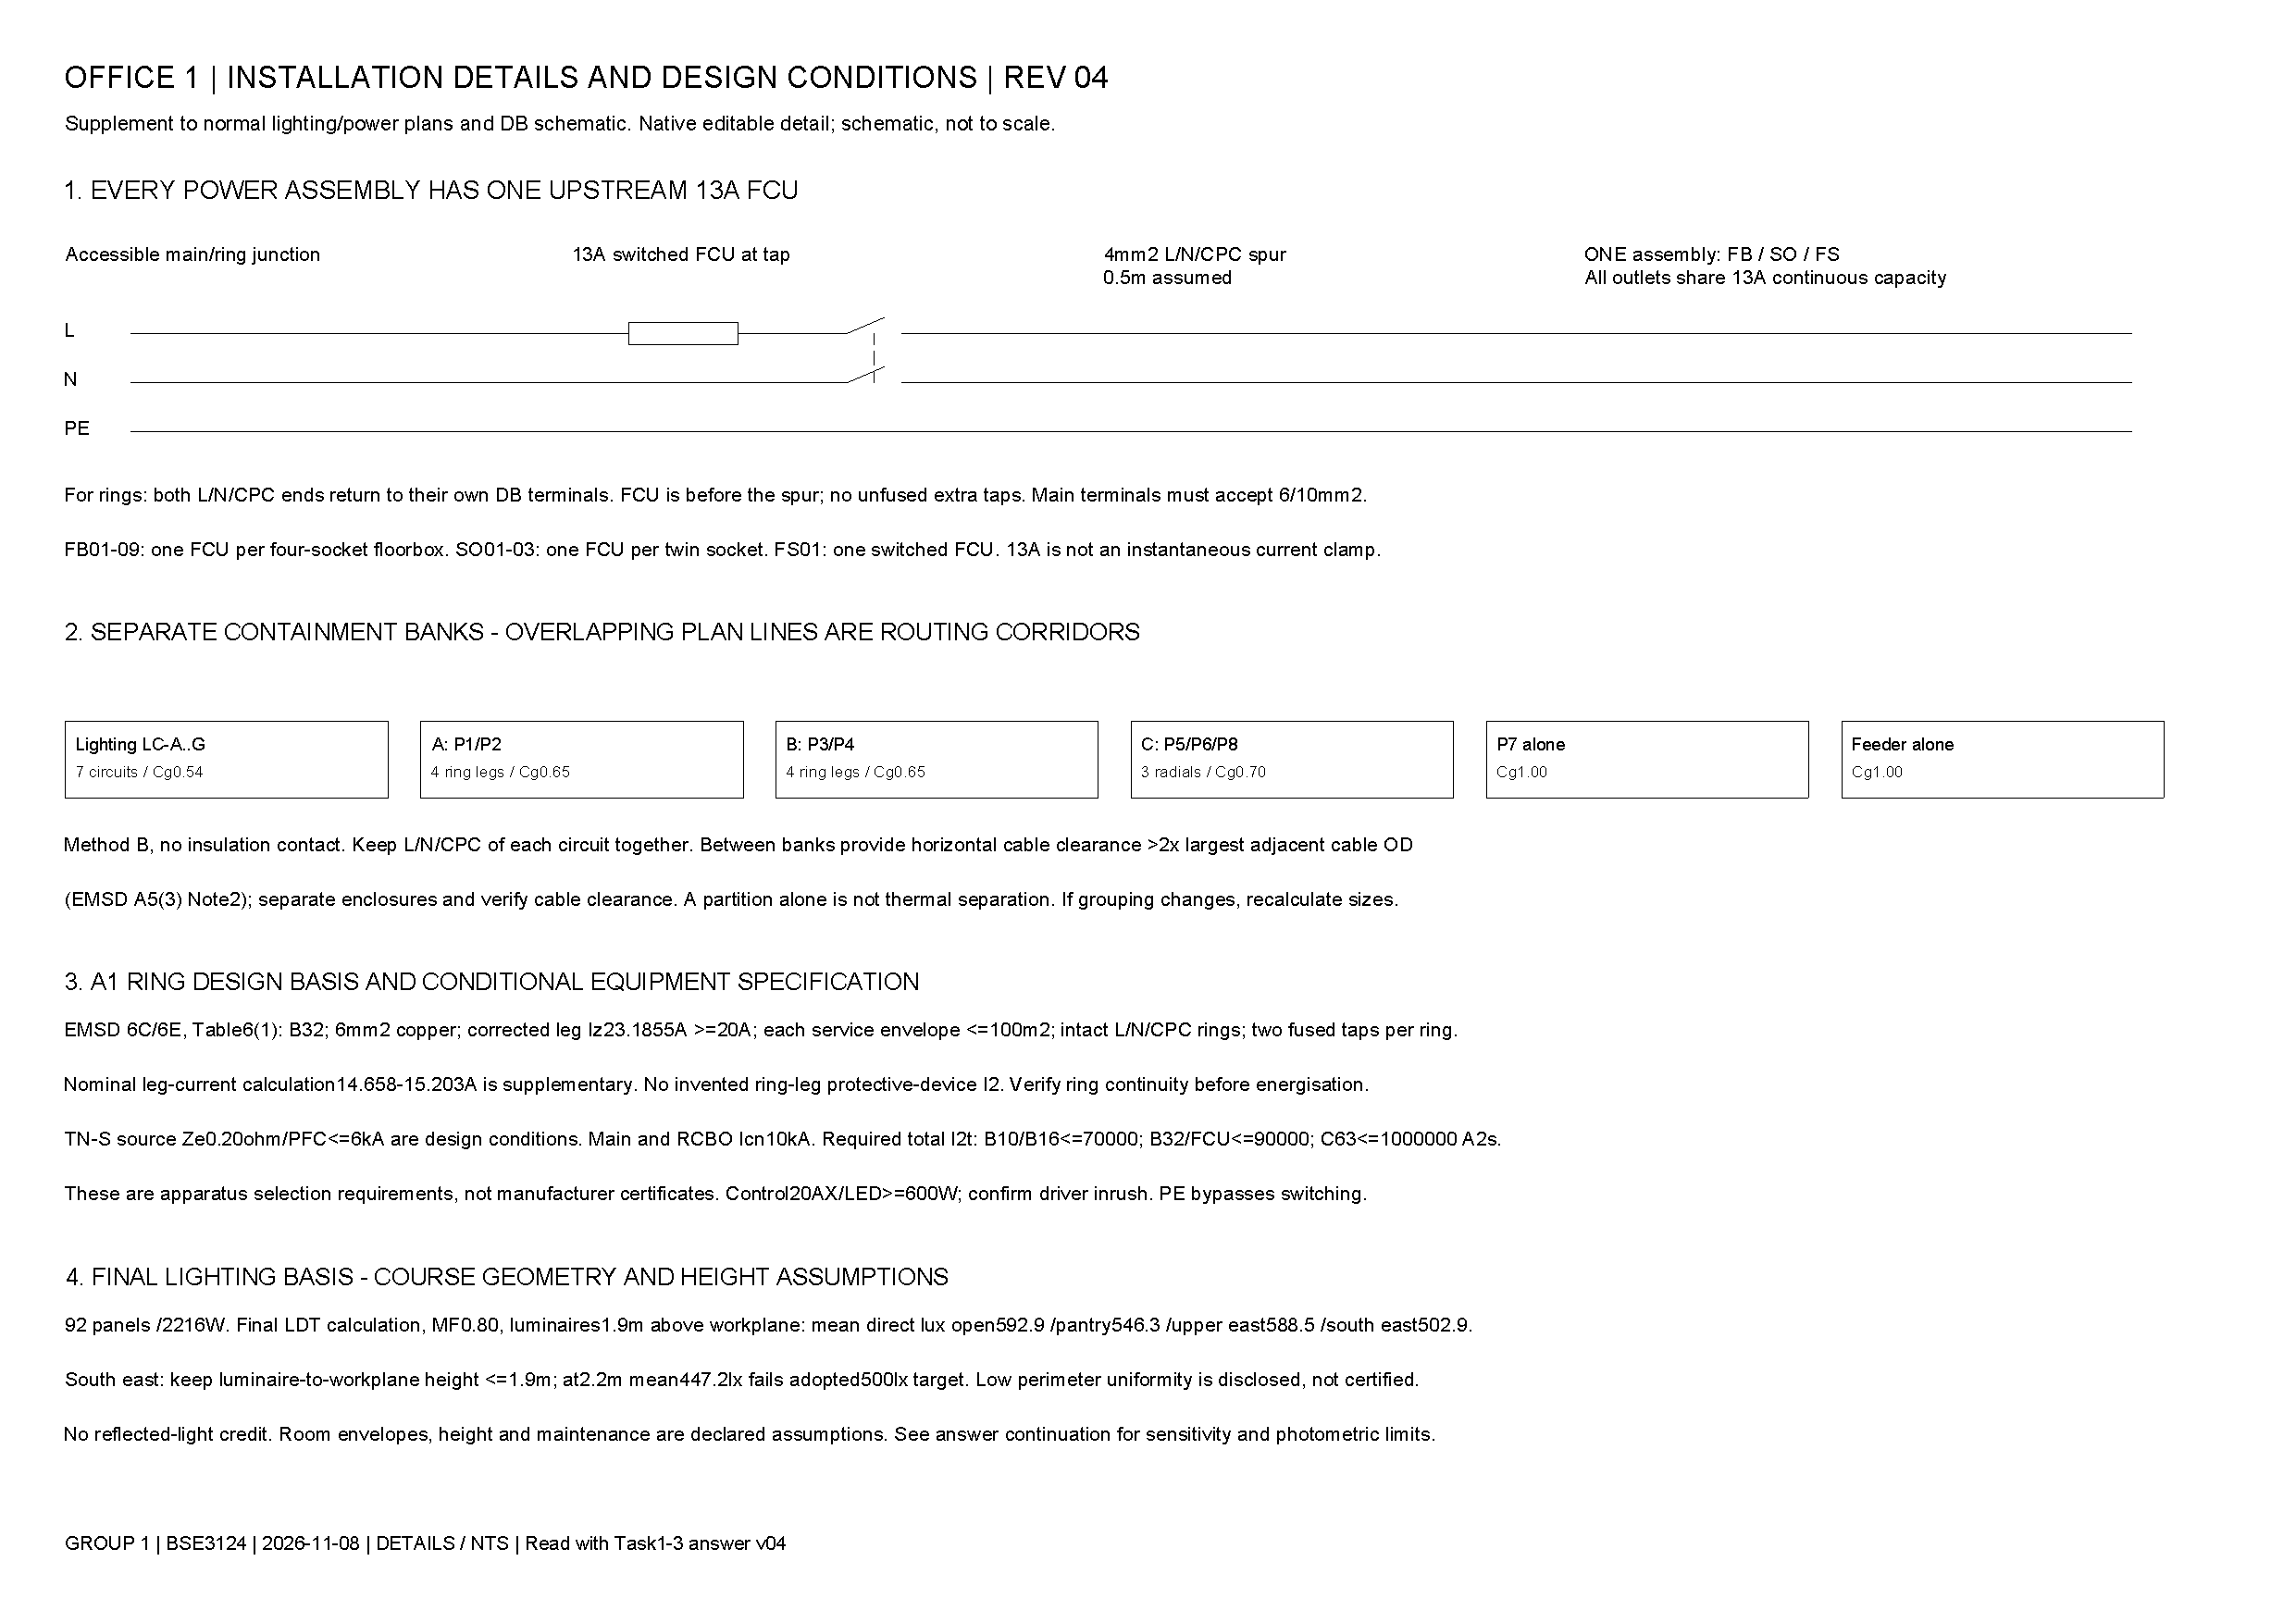
\includepdf[pages=-,fitpaper=true]{assets/installation-details.pdf}
\end{document}